%%%%%%%%%%%%%%%%%%%%%%%%%%%%%%%%%%%%%%%%%%%%%%%%%%%%%%%%%%%%%%%%%%%%%%%%%%%%%%%%%%%%%%%%%%%%%%%
%%%%%%%%%%%%%%%%%%%%%%%%%%%%%%%%%%%%%%%%%%%%%%%%%%%%%%%%%%%%%%%%%%%%%%%%%%%%%%%%%%%%%%%%%%%%%%%
%% LaTeX-Beamer template for KIT design
%% by Erik Burger, Christian Hammer
%% title picture by Klaus Krogmann
%%
%% version 2.1
%%
%% mostly compatible to KIT corporate design v2.0
%% http://intranet.kit.edu/gestaltungsrichtlinien.php
%%
%% Problems, bugs and comments to
%% burger@kit.edu
%%
%%
%% Modified: 30.1.2013, Schwall

\documentclass[12pt]{beamer}

%% SLIDE FORMAT
\usepackage{templates/beamerthemekit}

%% german time format (e.g 30.1.2013)
\usepackage{datetime}
\usepackage{bbm} %% Used to denote the indicator function
%\usepackage[T1]{fontenc}
\usepackage{amsmath}
\usepackage{amssymb}
\usepackage{amsfonts}
\usepackage{amsthm}
\usepackage{graphicx}
\usepackage{color,psfrag}
\usepackage{subfig}

\newdateformat{germandate}{\THEDAY.\THEMONTH.\THEYEAR}
\newdateformat{americandate}{\THEMONTH/\THEDAY/\THEYEAR}

% use these packages for PCM symbols and UML classes
\usepackage{templates/tikzkit}
\usepackage{templates/tikzuml}
\usepackage{siunitx}

\usepackage{times}
\usepackage{tikz}


\usepackage[english]{babel}
\usepackage{csquotes}
\setquotestyle{american}
\usepackage[language=american,autocite=footnote,citestyle=authortitle,citetracker=true,backend=biber,babel=other]{biblatex}
\addbibresource{../refs.bib}

\usepackage{verbatim}
\usetikzlibrary{arrows,shapes}

\setbeamerfont{footnote}{size=\tiny}
%%%%%%%%%%%%%%%%%%%%%%%%%%%%%%%%%%%%%%%%%%%%%%%%%%%%%%%%%%%%%%%%%%%%%%%%%%%%%%%%%%%%%%%%%%%%%%%
%%%%%%%%%%%%%%%%%%%%%%%%%%%%%%%%%%%%%%%%%%%%%%%%%%%%%%%%%%%%%%%%%%%%%%%%%%%%%%%%%%%%%%%%%%%%%%%
% the presentation starts here

\usepackage{datetime}
\newdate{date}{03}{09}{2014}

% english vs. ngerman
\selectlanguage{english}

\title{Estimation-Throughput Tradeoff for Underlay Cognitive Radio Systems}
\subtitle{ICC 2015, London}

\author{A. Kaushik\inst{1}, \textbf{S.K. Sharma}\inst{2}, S. Chatzinotas\inst{2}, B. Ottersten\inst{2}, F. K. Jondral\inst{1}}
\institute{\inst{1}Communications Engineering Lab, Karlsruhe Institute of Technology (KIT), Germany,\\
\and
\inst{2}SnT - securityandtrust.lu, University of Luxembourg, Luxembourg, \\
}
\subtitle{ICC 2015, London}

%% insert date in correct format
\iflanguage{english}{
	\date{11 June 2015}
	}{
	\date{\germandate\today}
}

\institute{\inst{1}CEL, Karlsruhe Institute of Technology (KIT), Germany and \inst{2}SnT, University of Luxembourg, Luxembourg}



\newcommand{\e}[2]{{\mathbb E}_{#1}\left[ #2 \right]}
\newcommand{\s}[2]{{\frac{1}{{#1}}\sum_n^{#1}} {#2}}
\newcommand{\q}[2]{{\mathcal Q}_{#1}\left( #2 \right)}
\newcommand{\p}{\mathcal P}
\newcommand{\sub}[1]{_{\text{#1}}}
\newcommand{\pd}{\text{P}\sub{d}}
\newcommand{\pc}{\text{P}\sub{c}}
\newcommand{\pcd}{\bar{\text{P}}\sub{c}}
\newcommand{\pdd}{\bar{\text{P}}\sub{d}}
\newcommand{\preg}{P\sub{cont}}
\newcommand{\xreg}{x\sub{cont}}
\newcommand{\prcvd}{P\sub{rcvd}}
\newcommand{\yrcvd}{y\sub{rcvd}}
\newcommand{\ptran}{P\sub{tran}}
\newcommand{\xtran}{x\sub{tran}}
\newcommand{\pp}{P\sub{p}}
\newcommand{\ps}{P\sub{s}}
\newcommand{\yp}{y\sub{p}}
\newcommand{\ys}{y\sub{s}}
\newcommand{\nap}{w\sub{p}}
\newcommand{\nas}{w\sub{s}}
\newcommand{\ite}{\theta\sub{I}}
\newcommand{\rs}{R\sub{s}}
\newcommand{\ers}{\e{}{\rs}}
\newcommand{\gp}{g\sub{p}}
\newcommand{\gs}{g\sub{s}}
\newcommand{\ap}{\alpha\sub{p}}
\newcommand{\as}{\alpha\sub{s}}
\newcommand{\npp}{\sigma^2\sub{p}}
\newcommand{\nps}{\sigma^2\sub{s}}
\newcommand{\npu}{\Delta\sigma^2}
\newcommand{\fsam}{f\sub{s}}


% distribution functions
\newcommand{\fpreg}{F_{\preg}}
\newcommand{\fprcvd}{F_{\prcvd}}
\newcommand{\fpp}{F_{\pp}}
\newcommand{\frs}{F_{\rs}}
\newcommand{\fgs}{F_{\gs}}
\newcommand{\fgp}{F_{\gp}}

% density functions
\newcommand{\dprcvd}{f_{\prcvd}}
\newcommand{\dK}{f_{\gp \ap/\prcvd}}
\newcommand{\dpp}{f_{\pp}}
\newcommand{\dpreg}{f_{\preg}}
\newcommand{\drs}{f_{\rs}}
\newcommand{\dgp}{f_{\gp}}
\newcommand{\dgs}{f_{\gs}}


\newcommand{\fs}[2]{\fontsize{#1 pt}{#2}\selectfont}
\DeclareMathOperator*{\Pro}{Pr}
\DeclareMathOperator*{\maxi}{max}
\DeclareMathOperator*{\expec}{\mathbb{E}}
\DeclareMathOperator*{\gthan}{\ge}
\DeclareMathOperator*{\eqto}{=}
\DeclareMathOperator*{\cosi}{ci}
\DeclareMathOperator*{\sini}{si}
\DeclareMathOperator*{\iGamma}{\text{inv}-\Gamma}
\DeclareMathOperator*{\ncchi2}{\mathcal{X'}^2}
\DeclareMathOperator*{\invncchi2}{\text{}\mathcal{X'}^2}
\setbeamerfont{normal text}{size=\small}
\setbeamerfont{frametitle}{size=\large}

\hyphenation{under-estimation over-estimation}

% Position the text inside the frame
\usepackage[absolute,overlay]{textpos}

\addtobeamertemplate{footnote}{}{\vspace{1.0ex}}
\addtolength{\footnotesep}{-5mm} % change to 1mm

\begin{document}

\newcommand\FrameText[1]{%
  \begin{textblock*}{\paperwidth}(0pt,\textheight)
    \raggedright #1\hspace{.5em}
  \end{textblock*}}



%title page
\begin{frame}
	\titlepage
\end{frame}

%%%%%%%%%%%%%%%%%%%%%%%%%%%%%%%%%%%%%%%%%%%%%%%%%%%% Frame %%%%%%%%%%%%%%%%%%%%%%%%%%%%%%%%%%%%%%%%%%%%%%%%%%%%%%	
\begin{frame}{Contents}
	\fs{10}{15}
	\begin{itemize}	
		\item Problem Statement
		\item System Model 
		\item Estimation Model 
		\item Numerical Analysis
		\item Summary 
	\end{itemize}
\end{frame}


%%%%%%%%%%%%%%%%%%%%%%%%%%%%%%%%%%%%%%%%%%%%%%%%%%%% Frame %%%%%%%%%%%%%%%%%%%%%%%%%%%%%%%%%%%%%%%%%%%%%%%%%%%%%%       
\begin{frame}[t]{Problem Statement}
        \begin{overlayarea}{\textwidth}{4.4cm}
	\begin{center}
                \only<1>
		{
			\includegraphics[width = 0.45 \paperwidth]{../figures/CR_Scenario_Underlay}
		}
		\only<2>
		{
			\vspace{0.8cm}	
			\includegraphics[width = 0.45 \paperwidth]{../figures/Frame_Structure_grau_U.eps}
		}
        \end{center}
	\end{overlayarea}
        \only<1>{
		\fs{8}{8}
		Underlay System:	
		\begin{itemize}
			\item A power control mechanism is employed at the ST
			\item Knowledge of the channel between the PR and the ST is necessary at the ST 
		\end{itemize}	
		In a realistic scenario:
		\begin{itemize}
		\item Channel knowledge is not available at the ST, hence, needs to be estimated
		\item No knowledge of the primary system $\Rightarrow$ direct estimation of channel is not possible 
		\item Perfect knowledge of noise power is required 
		\end{itemize} 
	}
	\only<2->{
		\fs{8}{8}
		Contributions:
		\begin{itemize}
			\item We propose a estimation model that estimates the received power at the ST $\implies$ channel knowledge
			\item We include the effect of noise uncertainty on the performance of the system $\implies$ best and worst case bounds 
			\item Based on analytical expressions, we characterize the performance of the system 
			\item We establish an estimation-throughput tradeoff and use it optimize the performance of the underlay system 
		\end{itemize}
	}
\end{frame}

%%%%%%%%%%%%%%%%%%%%%%%%%%%%%%%%%%%%%%%%%%%%%%%%%%%% Frame %%%%%%%%%%%%%%%%%%%%%%%%%%%%%%%%%%%%%%%%%%%%%%%%%%%%%%       
\begin{frame}{Assumptions and Considerations}
        \begin{columns}
                \begin{column}{0.5 \paperwidth}
                        \begin{center}
                                \includegraphics[width = 0.38 \paperwidth]{../figures/CR_Scenario_Underlay}
                        \end{center}
                \end{column}
                \begin{column}{0.5 \paperwidth}
                        \begin{center}
                                \includegraphics[width = 0.42 \paperwidth]{../figures/Frame_Structure_grau_U}
                        \end{center}
                \end{column}
        \end{columns}
        \vspace{0.5cm}
        \begin{itemize}
                \fs{8}{10}
                \item Coherence time of the channel $\approx T$  
                \item Power control at the ST is done by listening to the beacon or neighbouring pilot channel sent by the PR $\implies$ Channel reciprocity 
                \item In each frame, the ST performs estimation of the received power followed by data transmission with controlled power 
                \item In listening mode, ST considers proper alignment of the PR transmissions $\implies$ no interference is encountered at the SR from the PR 
		\item Transmit power of the PR is known at the ST 
        \end{itemize}

\end{frame}


%%%%%%%%%%%%%%%%%%%%%%%%%%%%%%%%%%%%%%%%%%%%%%%%%%%% Frame %%%%%%%%%%%%%%%%%%%%%%%%%%%%%%%%%%%%%%%%%%%%%%%%%%%%%%       
\begin{frame}{System Model}
        \vspace{-0.5cm}
        \fs{8}{8}
        \begin{columns}[t]
                \begin{column}{0.4 \paperwidth}
        	\begin{center}
     		   	\includegraphics[width = 0.38 \paperwidth]{../figures/CR_Scenario_Underlay}
       		\end{center}
		\vspace{-0.4cm}
		\begin{itemize}
                     \item Received signal at the ST
			\begin{equation*}
				\yrcvd[n] = \sqrt{\gp \cdot \ap} \cdot \xtran[n] + \nas[n]
			\end{equation*}
                     \item Received signal at the PR
			\begin{equation*}
				\yp[n] = \sqrt{\gp \cdot \ap} \cdot \xreg[n] + \nap[n]
			\end{equation*}
                     \item Received signal at the SR 
			\begin{equation*}
				\yp[n] = \sqrt{\gp \cdot \ap} \cdot \xreg[n] + \nap[n]
			\end{equation*}
		\end{itemize}
                \end{column}
                \begin{column}{0.4 \paperwidth}
                \begin{itemize}
                        \item Power received at the ST 
			 \begin{align*}
				\prcvd = \s{\tau \fsam}{ |\sqrt{\gp \ap} \xtran[n] + \nas|^2}.
			\end{align*}
                        \item Controlled power at the ST
                        \begin{align*}
                        \preg = \s{(T - \tau) \fsam}{|\xreg[n]|^2}
                        \end{align*}
                        \item Power received at the PR and at the SR 
                	\begin{align*}
                       	\pp = \s{(T - \tau) \fsam}{|\yp[n]^2|} \\
			\ps = \s{(T - \tau) \fsam}{|\ys[n]^2|} 
                        \end{align*}
		\end{itemize}
                \end{column}
        \end{columns}
\end{frame}


%%%%%%%%%%%%%%%%%%%%%%%%%%%%%%%%%%%%%%%%%%%%%%%%%%%% Frame %%%%%%%%%%%%%%%%%%%%%%%%%%%%%%%%%%%%%%%%%%%%%%%%%%%%%%       
\begin{frame}[t]{Estimation Model}
	\begin{itemize}
	\fs{8}{8}
        \item Conventional Model
	\begin{itemize}
		\fs{8}{8}
		\item Power Control 
		     \begin{equation*}
			\pp = \gp \ap \preg \le \ite 
		     \end{equation*}
		\item Throughput at the SR 
		\begin{equation*}
			\e{\gs, \preg}{\rs} = \e{\gs, \preg}{\log_2 \left(1 + \frac{\gs \as \preg}{\nps} \right)}. 
		\end{equation*}
	\end{itemize} 
	\item Proposed Model 
        \only<1> 
	{
		\begin{itemize}
			\fs{8}{8}
			\item Power Control
			\begin{align*}
				\preg = \frac{\ite K}{\prcvd}, 
			\end{align*}
			\item Throughput at the SR
			\begin{equation*}
				\rs = \frac{T - \tau}{T} \log_2 \left(1 + \frac{\gs \as \preg }{\nps} \right) 
			\end{equation*}
			\item Constraint at PR
			\begin{equation*}
				\pc \ge \pcd.
			\end{equation*}
		\end{itemize}
	}
	\only<2>
	{
		\begin{itemize}
			\fs{8}{8}
			\item Optimization problem
			\begin{align*}
				\maxi_{\tau}  & \text{      } \e{\gs, \preg}{\rs(\tau)} \\
				\text{s.t.} & \text{ } \pc(\tau \fsam, \mu) = \p \left( \frac{\left| \pp - \e{}{\pp} \right|}{\e{}{\pp}} < \mu \right) \ge \pcd, \nonumber  
			\end{align*}
			\item Probability of confidence is given by 
			\begin{align*}
				\pc = \fpp\left( {(1 + \mu) \e{}{\pp}}\right)  - \fpp\left({(1 - \mu) \e{}{\pp}} \right). 
			\end{align*}
		\end{itemize}		
	}
	\end{itemize}
\end{frame}


%%%%%%%%%%%%%%%%%%%%%%%%%%%%%%%%%%%%%%%%%%%%%%%%%%%% Frame %%%%%%%%%%%%%%%%%%%%%%%%%%%%%%%%%%%%%%%%%%%%%%%%%%%%%%       
\begin{frame}{Numerical Analysis}
        \fs{8}{8}
       	     \begin{columns}[t]
        		\begin{column}{0.45 \paperwidth}
                        \vspace{0.1cm}
               	 	\renewcommand{\arraystretch}{1.3}
           		\begin{center}
            	        \begin{tabular}{c|c}
                    		Parameter & Value\\
                   	        \hline \hline
               		        $\fsam$  & \SI{1}{MHz} \\ \hline
                       		$T$ & $\SI{100}{ms}$ \\ \hline
                 	        $\ap$ & $\SI{100}{dBm}$ \\ \hline
                  	        $\as$ & $\SI{80}{dBm}$ \\ \hline
                  	        $\ite$ & $\SI{-110}{dBm}$ \\ \hline
                  	        $\ptran$ & $\SI{0}{dBm}$ \\ \hline
                  	        $\gamma$ & $\SI{0}{dB}$ \\ \hline
                  	        $\npu$ & $\pm \SI{3}{dB}$ \\ \hline
                  	        $\npp, \nps$ & $ \SI{-100}{dB}$ \\ \hline
                  	        $\pcd$ & $ 0.95$ \\ \hline
                  	        $\mu$ & 0.025 \\ \hline
                   	        \hline
          		    \end{tabular}
                	\end{center}
                \end{column}
        	\begin{column}{0.5 \paperwidth}
			\begin{center}
      			Estimation-Throughput tradeoff: Path Loss 
			\input{../figures/fig_thr_est_time_tradeoff_AWGN_pres}
			\centering
			\begin{tikzpicture}[scale=1]
			\node[anchor=south west,inner sep=0] (image) at (0,0)
			{
     				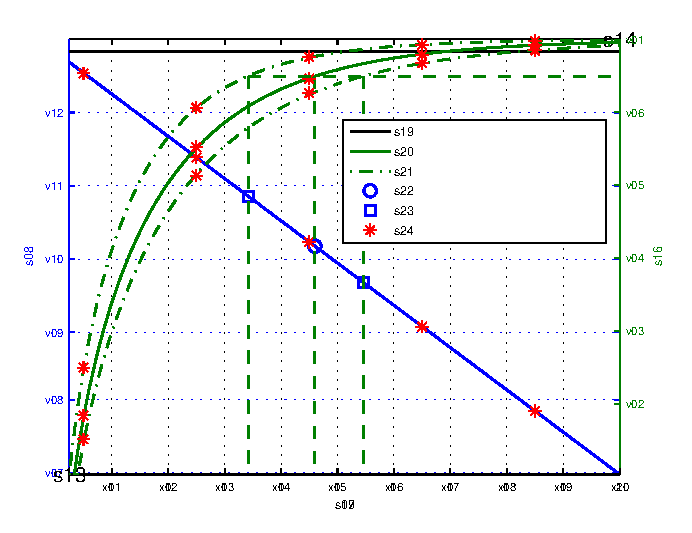
\includegraphics[width=0.9 \columnwidth]{../figures/fig_thr_est_time_tradeoff_AWGN_pres}
			};
			\begin{scope}[x={(image.south east)},y={(image.north west)}]
	
			% Select curves depending upon theta   
			\draw[black,->] (0.26,0.66) --  node[below=6.2mm, font=\tiny] {$\npu = \SI{3}{dB}$} (0.26,0.46);
			\draw[black,->] (0.26,0.80) --  node[above=1.7mm, font=\tiny] {$\npu = \SI{-3}{dB}$} (0.26,0.86);

			\draw(0.94,0.885) node[font=\tiny]{$\pcd$};
			\draw[black,<->] (0.465,0.545) --  node[left=0.0mm, font=\tiny] {$\beta$} (0.465,0.932);

			%\draw[help lines,xstep=.1,ystep=.1] (0,0) grid (1,1);
			%\foreach \x in {0,1,...,9} { \node [anchor=north] at (\x/10,0) {0.\x}; }
%\foreach \y in {0,1,...,9} { \node [anchor=east] at (0,\y/10) {0.\y}; }
			\end{scope}
		\end{tikzpicture}
		\end{center}
       		\end{column}	
	\end{columns}
	\vspace{0.5cm}
        \begin{itemize}
        \item For $\npu = \SI{-3}{dB}$, the probability of confidence constraint is fullfilled at lower $\tau$ 
        \end{itemize}
\end{frame}
	  
%%%%%%%%%%%%%%%%%%%%%%%%%%%%%%%%%%%%%%%%%%%%%%%%%%%% Frame %%%%%%%%%%%%%%%%%%%%%%%%%%%%%%%%%%%%%%%%%%%%%%%%%%%%%%       
\begin{frame}{Numerical Analysis}
        \fs{8}{8}
        \begin{columns}[t]
        \begin{column}{0.5 \paperwidth}
        \begin{center}
        Optimum throughput versus $\gamma$
		\input{../figures/fig_opt_thr_vs_snr_AWGN_pres}
		\centering
		\begin{tikzpicture}[scale=1]
		\node[anchor=south west,inner sep=0] (image) at (0,0)
		{
		        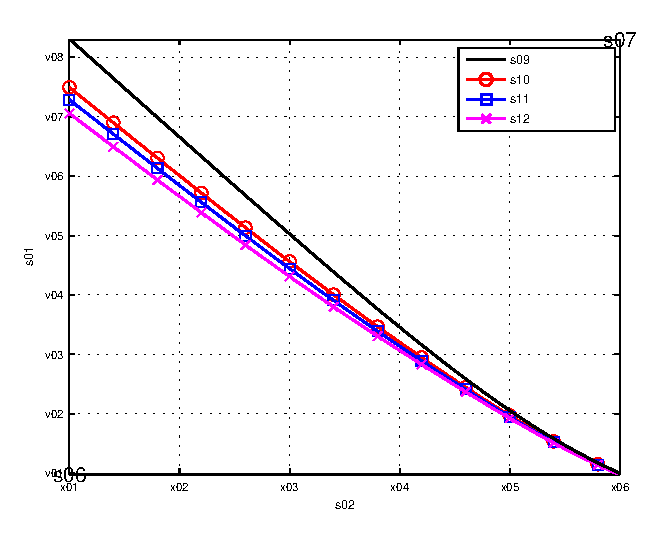
\includegraphics[width= 0.9 \columnwidth]{../figures/fig_opt_thr_vs_snr_AWGN_pres}
		};
		\begin{scope}[x={(image.south east)},y={(image.north west)}]

		% Select curves depending upon theta   
		%\draw[help lines,xstep=.1,ystep=.1] (0,0) grid (1,1);
		%\foreach \x in {0,1,...,9} { \node [anchor=north] at (\x/10,0) {0.\x}; }
		%\foreach \y in {0,1,...,9} { \node [anchor=east] at (0,\y/10) {0.\y}; }
		\end{scope}
	\end{tikzpicture}
        \end{center}
        \end{column}
        \begin{column}{0.5 \paperwidth}
        \begin{center}
        Optimum throughput versus Accuracy	
	\input{../figures/fig_opt_thr_vs_acc_AWGN_pres}
        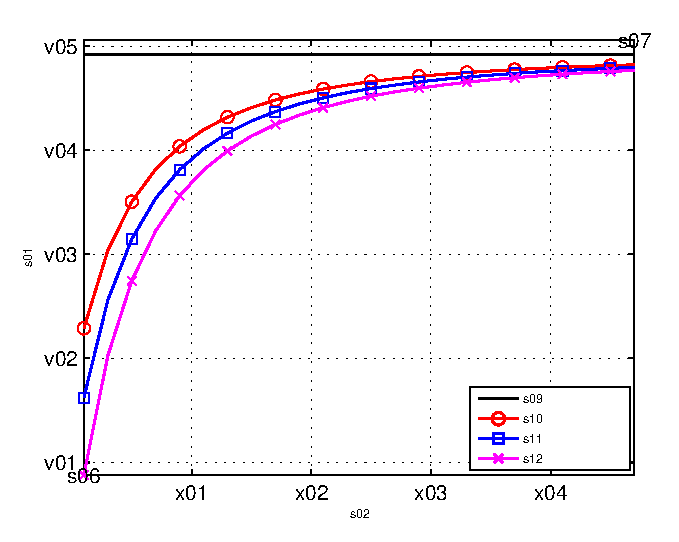
\includegraphics[width=0.925 \columnwidth]{../figures/fig_opt_thr_vs_acc_AWGN_pres}
	\end{center}
        \end{column}
        \end{columns}
        \vspace{0.5cm}
        \begin{itemize}
        \fs{8}{10}
        \item The variation in $\ap \in [85,110]$ \SI{}{dB} translates to the variation in $\gamma$. 
        \item At a given $\gamma = \SI{0}{dB}$, an improvement in PU performance (high $\mu$) leads to reduction in SU performance ($\ers$) 
        \end{itemize}
\end{frame}


%%%%%%%%%%%%%%%%%%%%%%%%%%%%%%%%%%%%%%%%%%%%%%%%%%%% Frame %%%%%%%%%%%%%%%%%%%%%%%%%%%%%%%%%%%%%%%%%%%%%%%%%%%%%%       
\begin{frame}[t]{Numerical Analysis}
        \vspace{0.5cm}
	\fs{8}{8}
        %\begin{columns}
        %\begin{column}{0.5 \paperwidth}
        %\begin{center}
	%\end{center}
        %\end{column}
        %\begin{column}{0.5 \paperwidth}
        \begin{center}
      	Estimation-Throughput tradeoff: Rayleigh Fading \\ 
	\input{../figures/fig_thr_est_time_tradeoff_fading_pres.tex}
	\centering
	\begin{tikzpicture}[scale=1]
		\node[anchor=south west,inner sep=0] (image) at (0,0)
		{
        	%% eps trial
    		   	 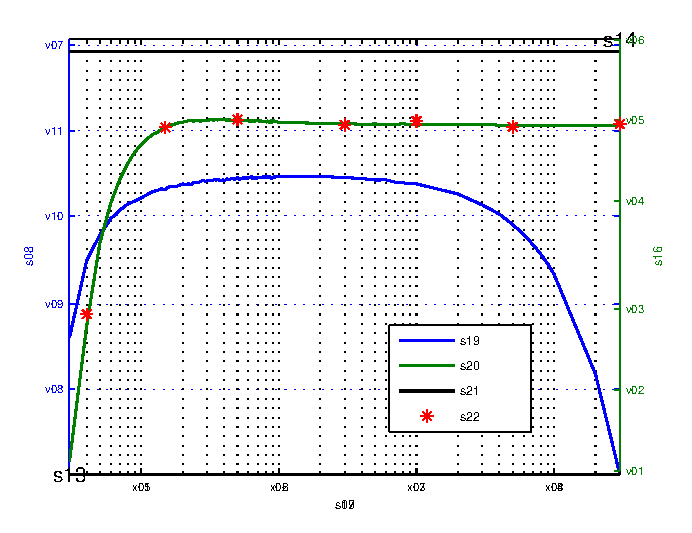
\includegraphics[width= 0.45 \columnwidth]{../figures/fig_thr_est_time_tradeoff_fading_pres.eps}
		};
		\begin{scope}[x={(image.south east)},y={(image.north west)}]

		% Select curves depending upon theta   
     		\draw[black,<->] (0.110,0.86) --  node[above = 0.0mm, font=\tiny] {Est. dominant} (0.31,0.86);
                \draw[black,<->] (0.315,0.86) --  node[above = 0.0mm, font=\tiny] {Channel dominant} (0.89,0.86);
		\draw[black,<->] (0.4,0.682) --  node[right=0.0mm, font=\tiny] {$\beta$} (0.4,0.927);

		%\draw[help lines,xstep=.1,ystep=.1] (0,0) grid (1,1);
		%\foreach \x in {0,1,...,9} { \node [anchor=north] at (\x/10,0) {0.\x}; }
		%\foreach \y in {0,1,...,9} { \node [anchor=east] at (0,\y/10) {0.\y}; }
		\end{scope}
	\end{tikzpicture}
	\end{center}
        %\end{column}
        %\end{columns}
		\begin{itemize}
       		\fs{8}{10}
     		\item In the estimation dominant regime $\tau < \SI{30}{\us}$, the system shows a improvement in $\pc$ with increase in $\tau$ 
       		\item In the channel dominant regime $\tau > \SI{30}{\us}$, $\pc$ reaches a saturation
		\item The variations in $\pp$ are mainly because of channel. Unlike the path loss channel, increasing $\tau$ doesn't improve the performance of the system 
       		\end{itemize}
\end{frame}


%%%%%%%%%%%%%%%%%%%%%%%%%%%%%%%%%%%%%%%%%%%%%%%%%%%% Frame %%%%%%%%%%%%%%%%%%%%%%%%%%%%%%%%%%%%%%%%%%%%%%%%%%%%%%
\begin{frame}{Summary}
\fs{8}{8}
\begin{itemize}
        \item Conclusion
        \begin{itemize}
        \fs{8}{10}
        \item To employ power control, we include channel estimation at the ST 
	\item We captured the variations induced due to the estimation process and characterize the performance of underlay system 
        %\item We investigated a tradeoff between the estimation time and expected throughput at the SR. 
        \item For the fading model, it was observed that $\pc$ is not a suitable choice for the PR constraint. 
        \item Finally, it is demonstrated via numerical analysis that the conventional model overestimates the performance of the underlay system 
        \end{itemize}
        \item Future Scope
        \begin{itemize}
        \fs{8}{10}
	\item We would like to investigate the performance of the system subject to outage probability constraint 
        \end{itemize}
\end{itemize}
\end{frame}


%%%%%%%%%%%%%%%%%%%%%%%%%%%%%%%%%%%%%%%%%%%%%%%%%%%% Frame %%%%%%%%%%%%%%%%%%%%%%%%%%%%%%%%%%%%%%%%%%%%%%%%%%%%%%	
\begin{frame}{}
\begin{center}
Thank you for attention! 
\end{center}
\end{frame}

%\printbibliography

\end{document}
